\documentclass[paper=a4, fontsize=11pt]{scrartcl} % A4 paper and 11pt font size

\usepackage[T1]{fontenc} % Use 8-bit encoding that has 256 glyphs
\usepackage{fourier} % Use the Adobe Utopia font for the document - comment this line to return to the LaTeX default
\usepackage[english]{babel} % English language/hyphenation
\usepackage{amsmath,amsfonts,amsthm,amssymb} % Math packages

\usepackage{algorithm, algorithmic}
\renewcommand{\algorithmicrequire}{\textbf{Input:}} %Use Input in the format of Algorithm  
\renewcommand{\algorithmicensure}{\textbf{Output:}} %UseOutput in the format of Algorithm  

\usepackage{graphicx}

\usepackage{listings}
\lstset{language=Matlab}

\usepackage{lipsum} % Used for inserting dummy 'Lorem ipsum' text into the template

\usepackage{sectsty} % Allows customizing section commands
\allsectionsfont{\centering \normalfont\scshape} % Make all sections centered, the default font and small caps

\usepackage{fancyhdr} % Custom headers and footers
\pagestyle{fancyplain} % Makes all pages in the document conform to the custom headers and footers
\fancyhead{} % No page header - if you want one, create it in the same way as the footers below
\fancyfoot[L]{} % Empty left footer
\fancyfoot[C]{} % Empty center footer
\fancyfoot[R]{\thepage} % Page numbering for right footer
\renewcommand{\headrulewidth}{0pt} % Remove header underlines
\renewcommand{\footrulewidth}{0pt} % Remove footer underlines
\setlength{\headheight}{13.6pt} % Customize the height of the header

\numberwithin{equation}{section} % Number equations within sections (i.e. 1.1, 1.2, 2.1, 2.2 instead of 1, 2, 3, 4)
\numberwithin{figure}{section} % Number figures within sections (i.e. 1.1, 1.2, 2.1, 2.2 instead of 1, 2, 3, 4)
\numberwithin{table}{section} % Number tables within sections (i.e. 1.1, 1.2, 2.1, 2.2 instead of 1, 2, 3, 4)

\setlength\parindent{0pt} % Removes all indentation from paragraphs - comment this line for an assignment with lots of text

%----------------------------------------------------------------------------------------
%	TITLE SECTION
%----------------------------------------------------------------------------------------

\newcommand{\horrule}[1]{\rule{\linewidth}{#1}} % Create horizontal rule command with 1 argument of height

\title{	
\normalfont \normalsize 
\textsc{Shanghai Jiao Tong University, UM-SJTU JOINT INSTITUTE} \\ [25pt] % Your university, school and/or department name(s)
\horrule{0.5pt} \\[0.4cm] % Thin top horizontal rule
\huge Mechatronic Systems Design\\ HW3 \\ % The assignment title
\horrule{2pt} \\[0.5cm] % Thick bottom horizontal rule
}

\author{Yu Cang \quad 018370210001} % Your name

\date{\normalsize \today} % Today's date or a custom date

\begin{document}

\maketitle % Print the title

\section*{Problem1}
	\begin{itemize}
		\item Q: Investigate and explain the coding for the disk of an absolute encoder.
		
		\item A: Inside an absolute encoder, there're serval concentric tracks on the code disk.
				 Each track represents a bit, combining these bits yields a digital word. 
		Each digital word corresponds to a unique rotational position of the shaft. 
		Thus, the absolute position of the shaft can be identified easily.\\
		The most common types of numerical encoding used are gray and natural binary codes. Natural binary code is straight forward but may suffer from mutiple changes of bits in one transition. Usually, the gray code is preferred as only one bit changes state for each count transition. 
		
	\end{itemize}

\section*{Problem2}
	\begin{itemize}
		\item 
			Q: Investigate and explain how does the hall sensors in the ABS work to measure the wheel velocity in a reasonable accuracy? Note that the sensor is essentially a low-resolution position sensor.
		
		\item 
			A: A typical configuration is shown as Fig(\ref{fig:hall}). Each time a gear teeth is opposed to the magnet, a peak voltage is generated. Thus the velocity can be measured from the gap between two pulse. Despite the low-resolution property of hall sensor, the velocity accuracy is refined by increasing the number of teeth when the radius of gear is fixed.
			
			\begin{figure}[!htbp]
				\centering
				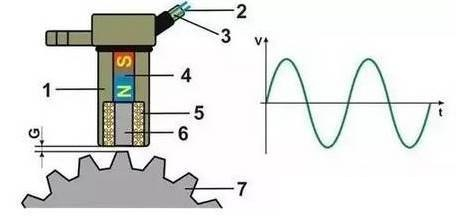
\includegraphics{hall.jpeg}
				\caption{Hall sensor in ABS}
				\label{fig:hall}
			\end{figure}

		
	\end{itemize}

\end{document}
